\section{Flat processing schemes vs. deep hierarchies}
\label{sec:deep_hierarchies}
In the SIFT object recognition algorithm an object is identified
by obtaining features known as keys, in an input image,
followed by a search for these features in a database.
When multiple statements point at a specific object,
further effort will be made to specify it, and eventually an object will be identified,
given that it is in the database \citep{sift}.
The complexity of this unbounded visual search (referred to as a flat processing scheme)
is NP complete \citep{fidler2009learning}.

In figure \ref{fig:deepvsflat}, on the right is shown a graphical representation of the flat processing scheme,
where each task oriented algorithm computes with respect to a big database of known features.
On the left is the representation of a hierarchal structure where common computations are made to support multiple tasks,
hereby sharing information.

\begin{figure}[h!] %fancyboxes
\centering
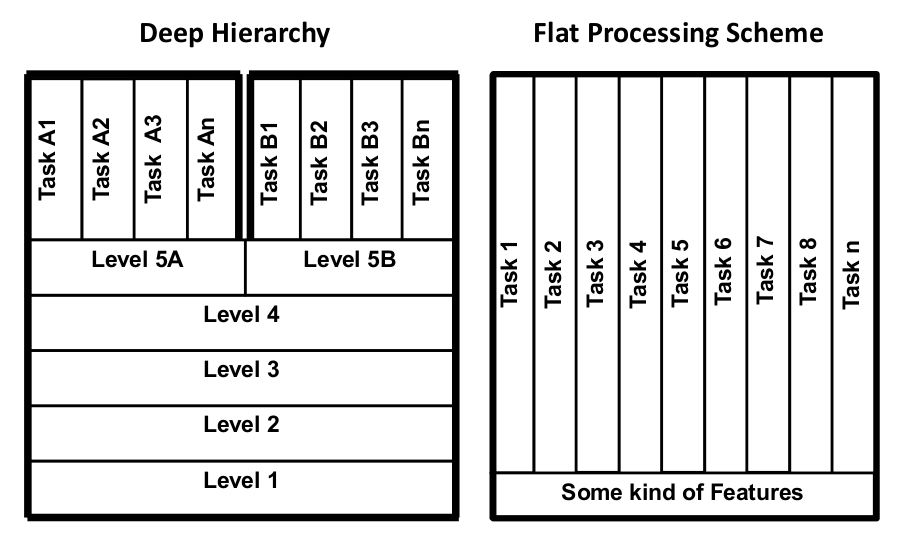
\includegraphics[width=0.6\textwidth]{graphics/deepvsflat}
\caption[Deep hierarchies and flat processing schemes]{Deep hierarchies and flat processing schemes 
\citep[fig.~1]{kruger2013deep}. } 
\label{fig:deepvsflat}
\end{figure}

As will be discussed in section \ref{sec:pvc}, the primate visual system
is a deep hierarichal network, and this could mean that
computer vision systems built using deep hierarichal networks could
be a more optimized way to develop robust systems, than using flat processing schemes.
As mentioned, the human brain seems to interpret visual stimuli with very little effort,
and therefore trying to emulate the brain of primates might help in optimizing object recognition in computer vision.
Especially the relatively recent development of multi-core systems in computer science
greatly supports the idea of these structures as parallel processing is of fundamental character in the primate brain.\citep{fidler2009learning}.

A hierarchical model consists of a number of layers placed “on top of each-other”.
Each item in a layer, representing more advanced features,
is composed of items from the layers below, which represent simpler features,
the smallest feature typically being an edge.

This form of representation gives some main advantages,
taking the aspect of computational efficiency and storage space into account.
As stated, layers of more advanced features are composed from elements of the layer below,
hence only the fundamental building blocks are directly stored,
along with information regarding connections of compositions.
In addition, this method takes advantage of the fact that some lower level items
will be reused in many of the items in layers above, which minimizes the need of duplicates.
With this form of representation, results presented in \citet{fidler2009learning} indicate that
only very few actual descriptors are needed: only six is used in the lowest layer,
and a few hundred in the other layers.
In fact, the best “flat processing schemes” of today must store millions of small images
with 25 x 25 pixels as descriptors in order to get satisfying results,
which is in great contrast to hierarchies \citep{fidler2009learning}.

Another advantage of the deep hierarchy is what is refereed to as generalization.
Generalization means that, like in the primal brain,
we can make common calculations applicable to several individual tasks
related to computer vision such as object recognition and categorization,
grasping, manipulation, path planning, etc. \citep{kruger2013deep}.
